

Da das Fließverhalten der Kunstoffe nur schwer abschätzbar ist, wird zur Erprobung ein vereinfachter Aufbau verwendet. In das Heizrohr ist ein Stahlrohr  eingeführt, welches das Original Keramik Innenrohr vor Verunreinigungen schützt. Die Probe wird Vertikal in das Rohr gehängt und Erwärmt, zu sehen in Abbildung \ref{fig:testaufbau}. Der Versuch soll Aufschluss über die nötige Abzugsgeschwindigkeit, Materialfördergeschwindigkeit und Form der Faser geben.


\begin{figure}[!h]
\centering
\begin{minipage}{.5\textwidth}
  \centering
  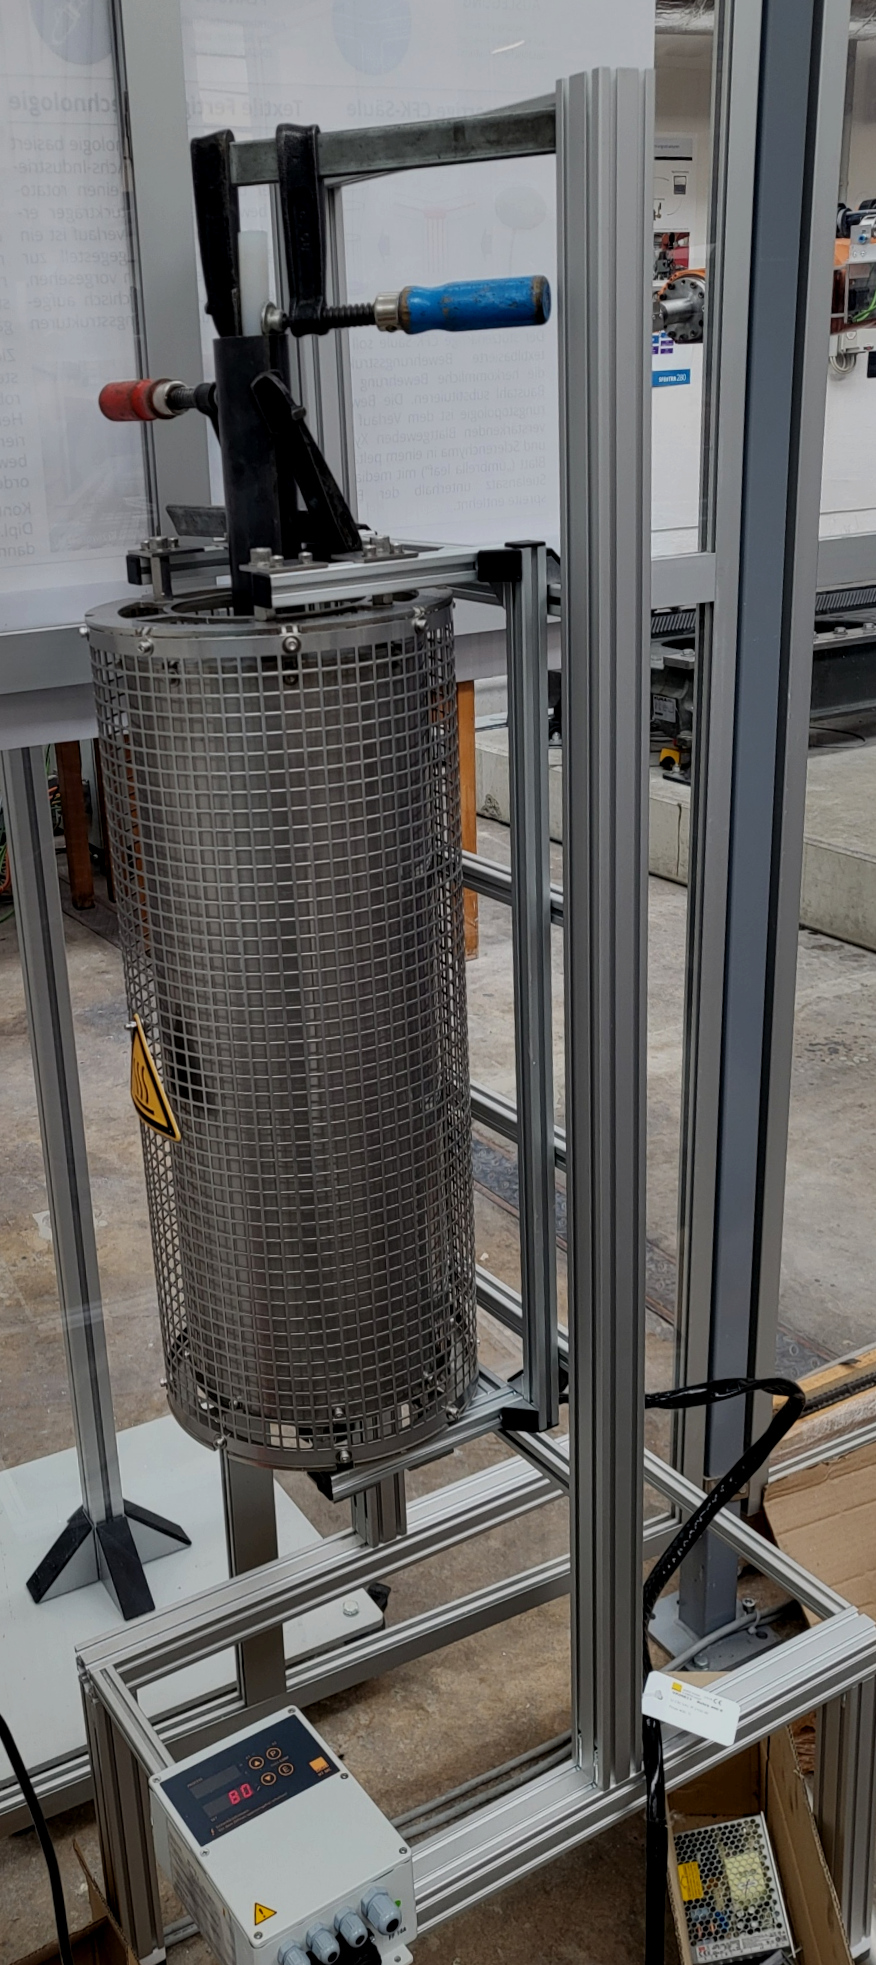
\includegraphics[width=.4\linewidth]{Abbildungen/Versuche/testaufbau_0010.jpg}
  \captionof{figure}{Testaufbau}
  \label{fig:testaufbau}
\end{minipage}%
\begin{minipage}{.5\textwidth}
  \centering
  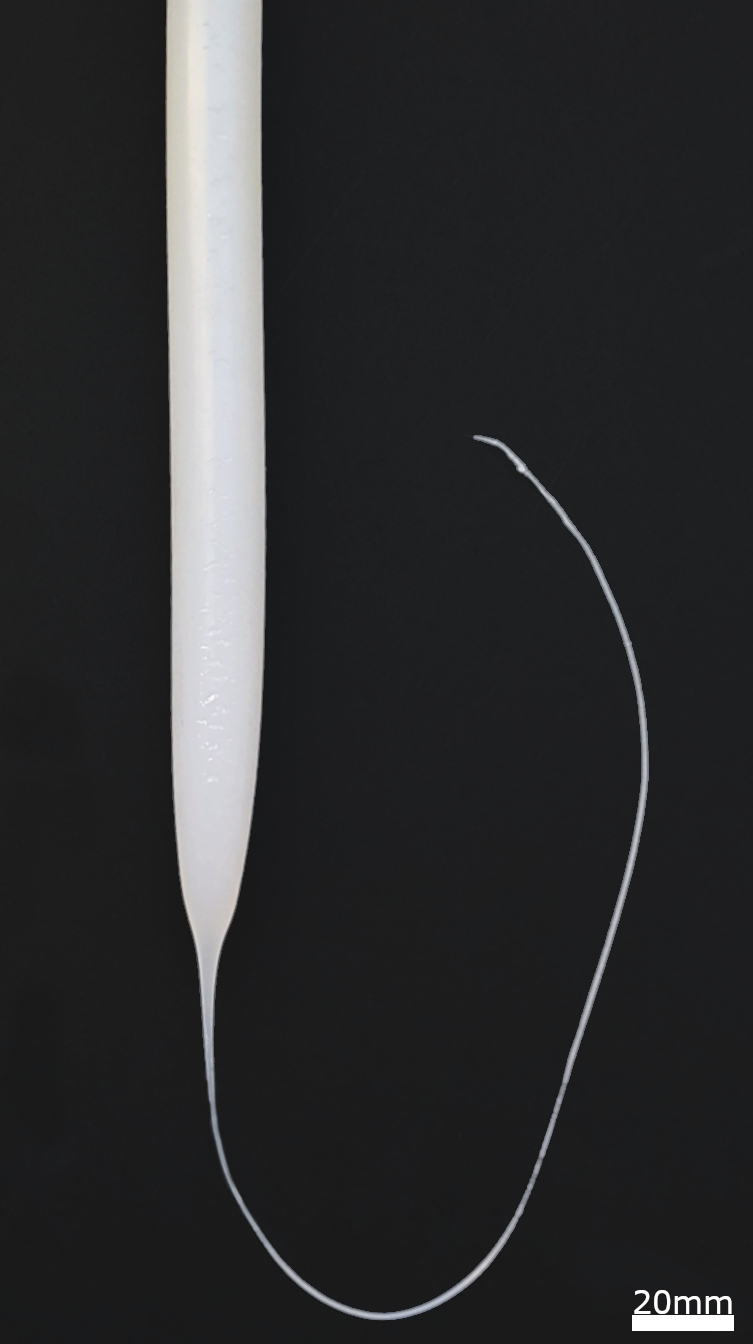
\includegraphics[width=.5\linewidth]{Abbildungen/Versuche/probe1_w.jpg}
  \captionof{figure}{\acs{evac}}
  \label{fig:probe1}
\end{minipage}
\end{figure}
 Die Erste Probe aus Abbildung \ref{fig:probe1} hat bei circa 205°C zu fließen begonnen. Dieser Versuch sollte nur veranschaulichen ob das gewählte Prinzip Funktionsfähig ist. Da sowohl die Faserdicke als auch die Fließform den erwartungen entsprechen, werden im nächsten Schritt andere Materialien verwendet. Um das Fließverhalten besser einschätzten zu können sind die folgenden Probenkörper mehrfarbig ausgeführt. Dadurch lässt sich beeurteilen wie die Faser aufgebaut ist. \newpage

 \begin{figure}[!h]
     \centering
     \begin{subfigure}[]{.29\textwidth}
         \centering
         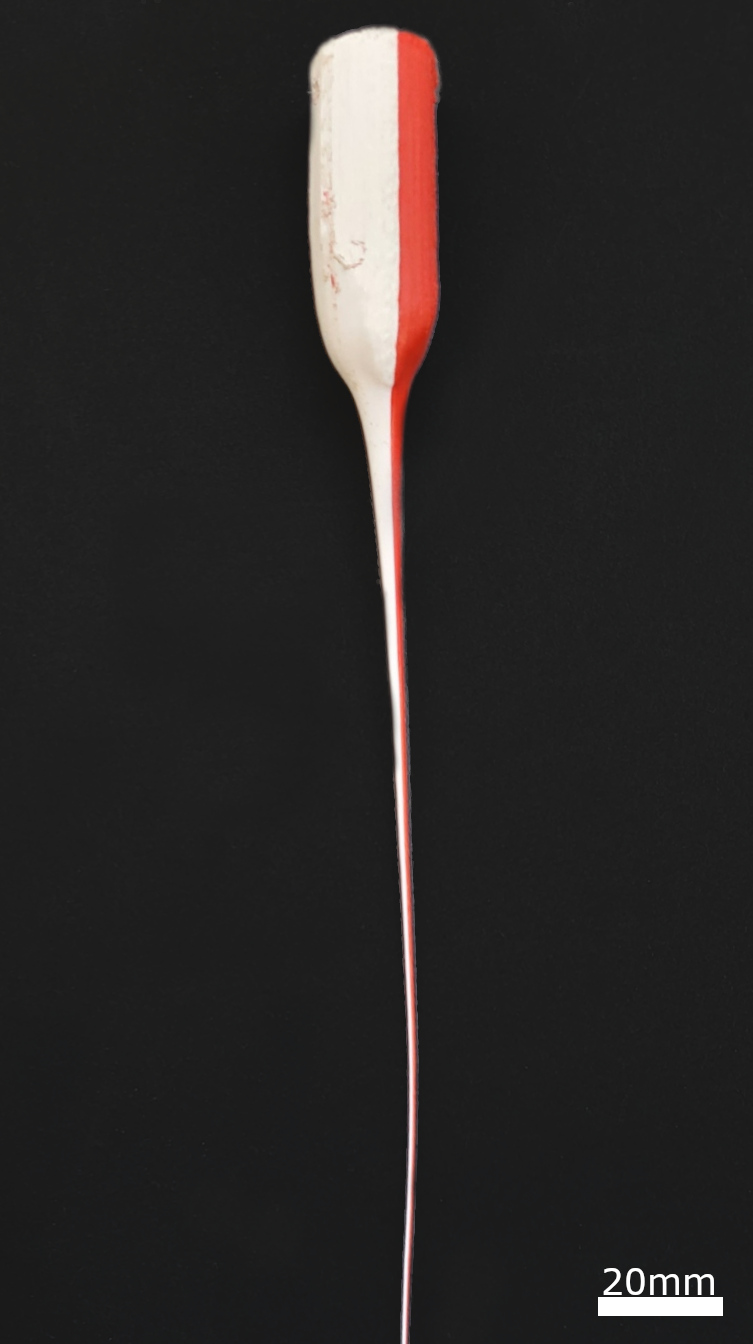
\includegraphics[width=\textwidth]{Abbildungen/Versuche/probe3_w.jpg}
         \caption{\acs{pla}/ \acs{pla}} 
         \label{fig:probe2}
     \end{subfigure}
     \hspace{5mm}
     \begin{subfigure}[]{.29\textwidth}
         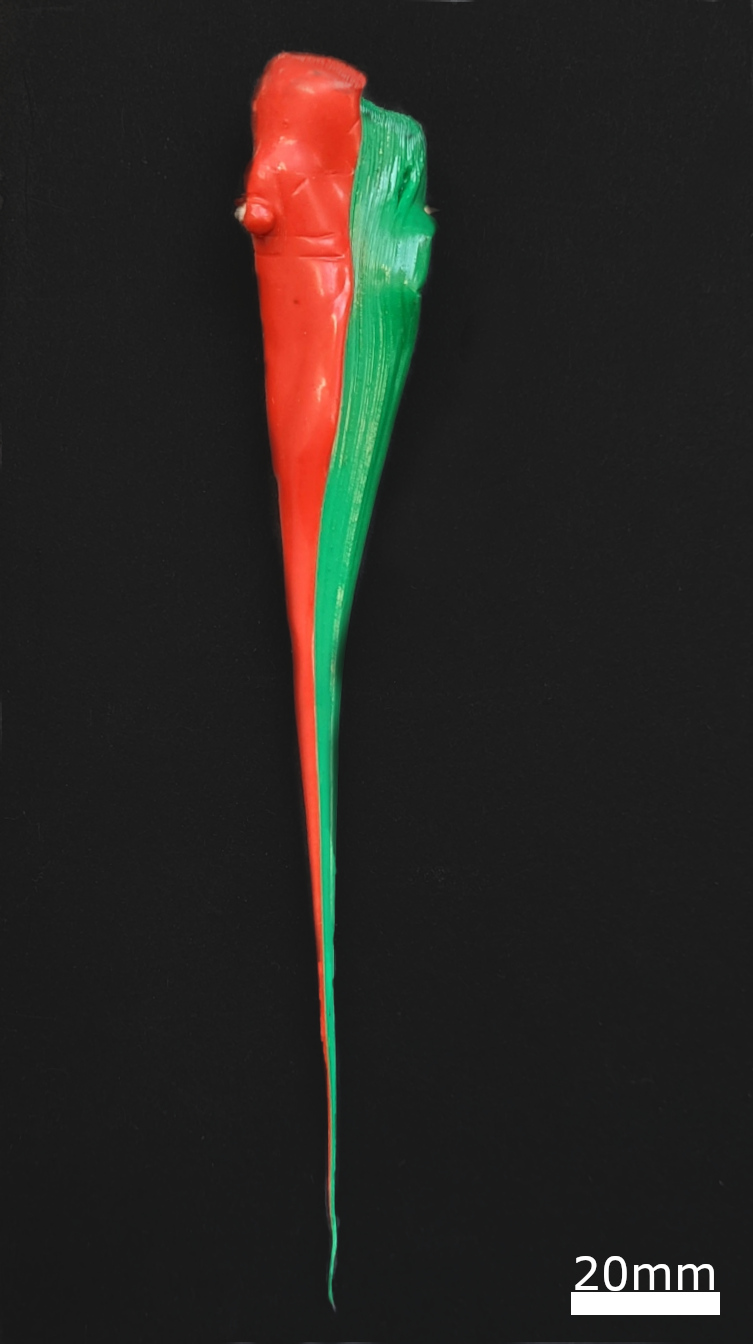
\includegraphics[width=\textwidth]{Abbildungen/Versuche/probe2_w.jpg}
         \caption{\acs{pla}/\acs{abs}}
         \label{fig:probe3}
     \end{subfigure}
     \hspace{5mm}
     \begin{subfigure}[]{.29\textwidth}
        \centering
        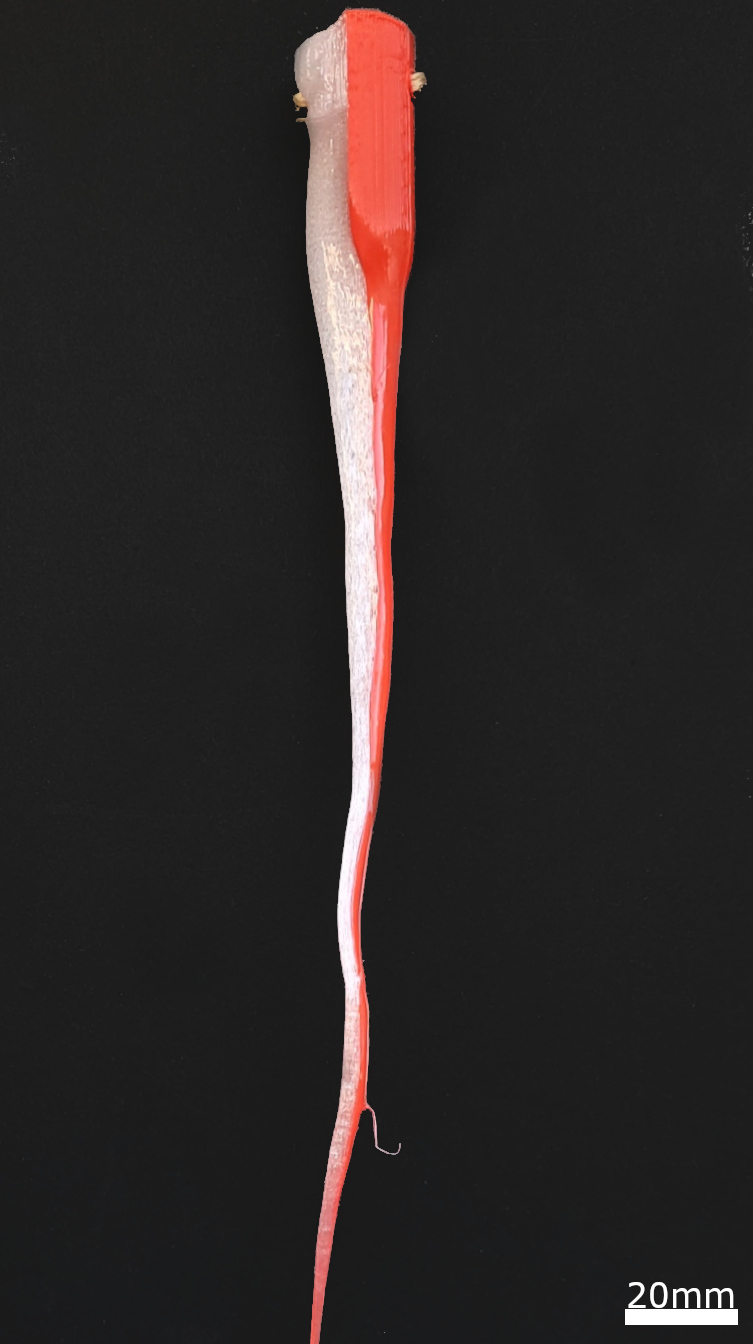
\includegraphics[width=\textwidth]{Abbildungen/Versuche/probe4_w.jpg}
         \caption{\acs{petg}/\acs{pla} }
        \label{fig:probe4}
     \end{subfigure}
     \caption{Probenkörper aus verschiedenen Materialkombinationen}
      \label{fig:probenkoerper_vor}
        \end{figure}

 \begin{figure}[!h]
     \centering
     \begin{subfigure}[]{.29\textwidth}
         \centering
         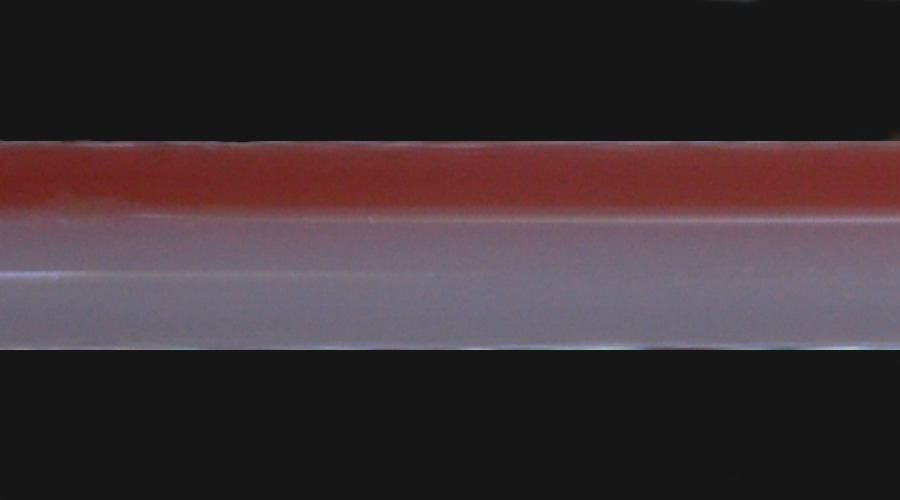
\includegraphics[width=\textwidth]{Abbildungen/Versuche/plapla_n.jpg}
         \caption{\acs{pla}/ \acs{pla}} 
         \label{fig:probe2_f}
     \end{subfigure}
     \hspace{5mm}
     \begin{subfigure}[]{.29\textwidth}
         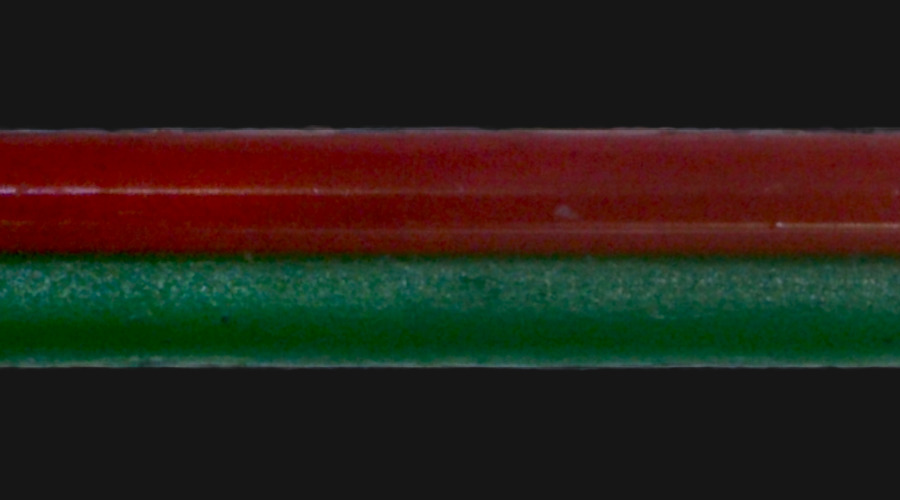
\includegraphics[width=\textwidth]{Abbildungen/Versuche/abspla_n.jpg}
         \caption{\acs{pla}/\acs{abs}}
         \label{fig:probe3_f}
     \end{subfigure}
     \hspace{5mm}
     \begin{subfigure}[]{.29\textwidth}
        \centering
        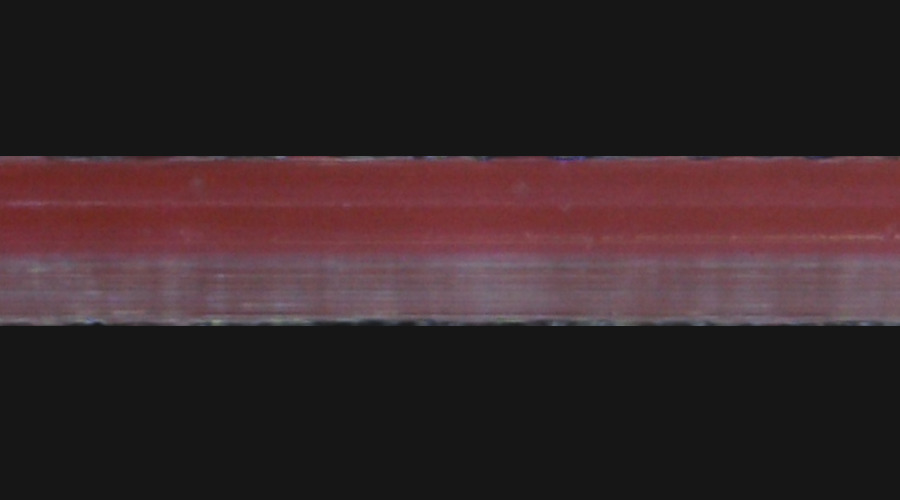
\includegraphics[width=\textwidth]{Abbildungen/Versuche/petgpla_n.jpg}
         \caption{\acs{petg}/\acs{pla} }
        \label{fig:probe4_f}
     \end{subfigure}
     \caption{Fasern aus verschiedenen Materialkombinationen}
      \label{fig:probenkoerper_vor}
        \end{figure}
    

Bei dem aktuell gewählten Prozess ist die Voraussetzung das sich beide Materialien des Probenkörpers, durch  erwärmen in ihrer Viskosität soweit herab gesenkt werden können das es ohne weiteren Eingriff in den Vorgang zu einer Ausbildung der Faser kommt. In der Zweiten Versuchsreihe sichtbar das dies zu problemen führen kann. In der Abbildung \ref{fig:probe2} wird ein Probenkörper aus zwei verschiedenen Farben \acs{pla} verwendet, was zum Ziel hatte das Erste Ergebnis zu replizieren und die Verteilung der Materialien zu beurteilen. Die Temperatur bei welcher sich der Prozess eingestellt hat liegt bei ca. 353°C. Dabei ist zu beachten das es sich bei der Angabe nicht um die Tatsächliche Materialtemperatur sondern um den Einstellwert des Rohrofens handelt. Die Materialtemperatur wurde nicht ermittelt, was jedoch während der Inbetriebnahme des gesamten Versuchsstandes und zur Stabilisierung des Prozesses in Betracht zu ziehen ist. Bei dieser Probe ist zu sehen das sich ein gleichmäßiger Abschmelzkegel (Abbildung \ref{fig:probe2}) sowie eine gleichmäßige Verteilung der \acs{pla}-Anteile (Abbildung \ref{fig:probe2_f}) ausbildet. Die ermittelte mittlere Faserdicke (Tabelle \ref{tab:erm_faserdicke}) ist ebenfalls inerhalb der Vorgaben. Anders als In Kapitel \ref{sec:therm} ist Sind die Probenkörper aus mehreren Materialien nicht mit einem stabil viskosem Mantel überzogen. So kann berurteilt werden ob dieser nötig ist oder ob es genügt wenn die Verarbeitungstemperaturen der Materialien eng beeinader liegen. In Abbildung \ref{fig:probe3} und \ref{fig:probe4} ist zu erkennen das der Abschmelzkegel sehr ungleichmäßig ist. Die Verabeitungstemperaturen von \acs{pla} und \acs{abs} liegen circa 30°C auseinader. Bei \acs{petg} und \acs{pla} sind es circa 40°C. Daraus lässt sich schließen das die Ausbildung eines gleichmäßigen Kegels maßgeblich von der Temperaturschere zwischen den gewählten Materialien abhängt. Das selbe Phänomen lässt sich auch bei der fertigen Faser erkennen. In Abbildung \ref{fig:probe3_f} ist zu sehen das die Verteilung der zwei Werkstoffe noch recht gleichmäßig ist, jedoch sind die zwei Halbzylinder nicht mehr vollständig an den Schnittfläche laminiert, was zu einer Sicke entlang der Grenzfläche führt. In Abbildung \ref{fig:probe4_f} ist die Temperaturdifferenz noch größer und so zeigt sich auch ein noch schlechteres Ergebnis. Zu sehen ist nur ein Dicke Schicht aus \ac{pla} mit einer ganz dünnen Anhaftung von \acs{petg}. Auch wenn die erreichten Dicken (Tabelle \ref{tab:erm_faserdicke}) innerhalb der Grenzwerte liegen ist das Ergebnis nicht Erwartungsgemäß. Da sich der Aufbau der Faser in den letzten zwei Versuchen nicht kontrollieren ließ ist es schwierig ein konstantes Ergebnis erzeugen, welches Später als Sensor oder Aktor verwendet werden kann.

\begin{center}
    \begin{table}[!h]
    \centering
        \begin{tabular}{c|c|c|c|c}
                Materialkombination & mittlere Dichte $\rho$ & Länge L & Masse m & Durchmesser d \\
                \hline
                \acs{pla}/\acs{pla} & $1,240 \frac{g}{cm^3}$ & $126 cm$ & $0,158g$ & $358\mu m$ \\
                \acs{pla}/\acs{abs} & $1,145 \frac{g}{cm^3}$ & $140 cm$ & $0,125g$ & $315\mu m$ \\
                \acs{petg}/\acs{abs} & $1,310 \frac{g}{cm^3}$ & $168 cm$ & $0,120g$ & $263\mu m$ \\
                
        \end{tabular}
        \\
        \begin{center}
            \begin{equation*}
                d = 2 \cdot \sqrt{\frac{m}{\rho * \pi * L}}
            \end{equation*}
        \end{center}
    \caption{Ermittelte Faserdicke}
    \label{tab:erm_faserdicke}
    \end{table}
\end{center}

Ein weiterer unbekannter Faktor ist die benötigte Abzugsgeschwindigkeit. Im Zuge einer Videoauswertung eines der Abzugsvorgänge konnte ein grober Richtwert von $72\frac{mm}{s}$ ermittelt werden.
Da es in dieser Studienarbeit mehr um die Entwicklung des Verfahrens und weniger um die Optimierung der Probenkörper geht sind die Erlangten Erkenntnisse sehr Hilfreich und bestätigen die Funktionsweise des Verfahrens grundsätzlich.
